\subsubsection{04.12.2015 (Competition)}
\textit{\textbf{Time frame:}} 8:00-22:00

Today was the first day of competition. There were only training matches, so we were just preparing robot for the qualifications.

\begin{figure}[H]
	\begin{minipage}[h]{0.31\linewidth}
		\center{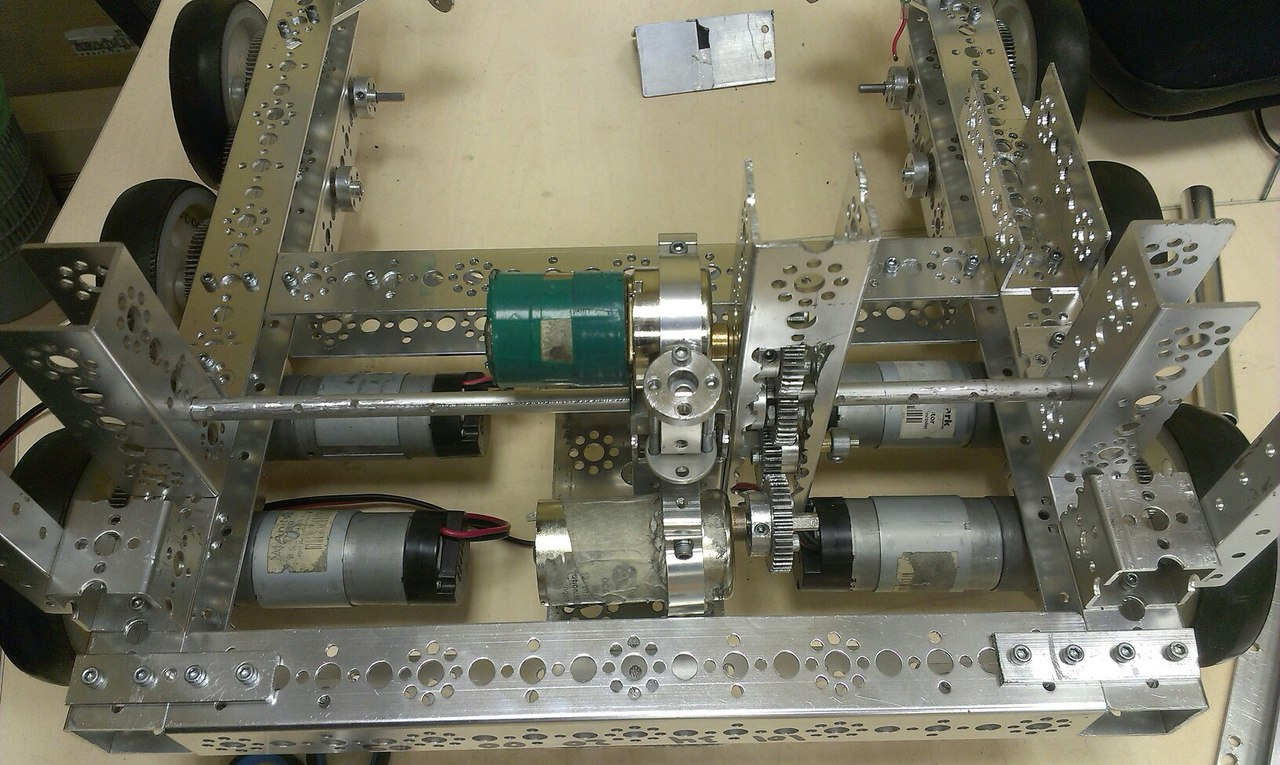
\includegraphics[scale=0.25]{3Engineering/5Team_meetings/days_of_meetings/2015.12.04/images/01}}
		\caption{Preparing robot 1}
	\end{minipage}
	\hfill
	\begin{minipage}[h]{0.31\linewidth}
		\center{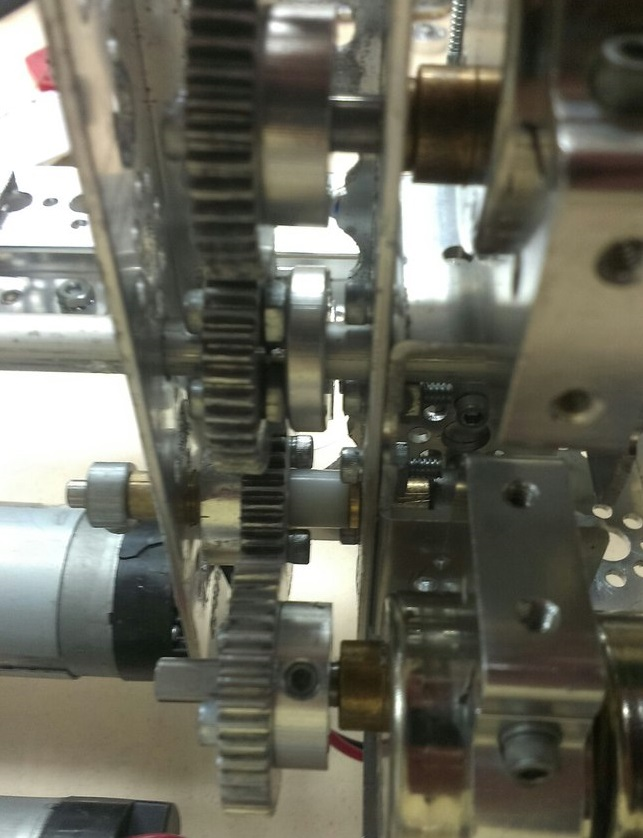
\includegraphics[scale=0.25]{3Engineering/5Team_meetings/days_of_meetings/2015.12.04/images/02}}
		\caption{Preparing robot 2}
	\end{minipage}
	\hfill
	\begin{minipage}[h]{0.31\linewidth}
		\center{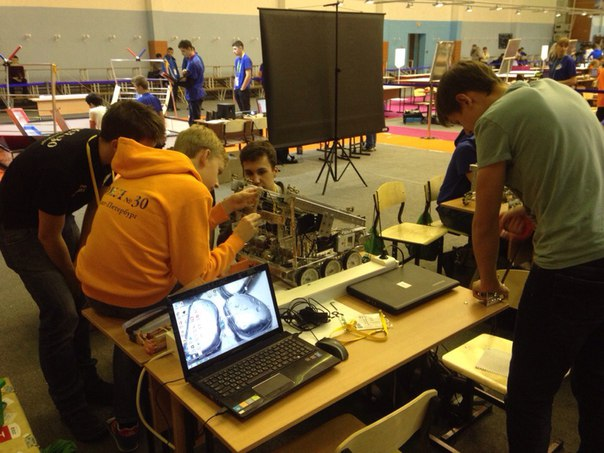
\includegraphics[scale=0.25]{3Engineering/5Team_meetings/days_of_meetings/2015.12.04/images/03}}
		\caption{Preparing robot 3}
	\end{minipage}
\end{figure}

Today the winch was tested for the first time, it was found out, that there is one weak point: the screw that connected the axis with motors carried too much load, so it broke down as soon as the winch started extracting the elevator. Unfortunately, it was a very severe mistake in development and all the mechanism became useless without the connection between motors and coils.

Due to this, the mechanism was totally disassembled. After that, it was decided to create a temporary mechanism for extracting of the elevator for the competition "Robofest South", that took place the next day. There were created two independent coils, powered by one motor each. This construction was also tested, but due to both coils were not synchronised, two sides of the elevator were extracting with different speed and it could break the slats. That's why it was decided to not to use this system at the competition.